\documentclass{article}
\usepackage[english]{babel}
\usepackage[letterpaper,top=2cm,bottom=2cm,left=3cm,right=3cm,marginparwidth=1.75cm]{geometry}
\usepackage{amsmath}
\usepackage{graphicx}
\usepackage{algorithm2e}
\usepackage{forest}
\usepackage{tikz}
\usepackage[colorlinks=true, allcolors=blue]{hyperref}

\title{\textbf{CS456: Algorithm Design and Analysis}}
\author{Elikem Asudo Tsatsu Gale-Zoyiku}
\date{\today}

\begin{document}
\maketitle
\begin{center}
    \begin{large}
        \textbf{Assignment 4\\}
    \end{large}
\end{center}
\newpage

\section*{Problem 1 (Prim's Algorithm)}
\begin{table}[ht]
    \centering
    \begin{tabular}{|c|c|}
        \hline
        \textbf{Tree Vertices} & \textbf{Remaining Vertices}                                                                                                          \\
        \hline
        a(-,-)                 & b(a,3) c(a,5) d(a,4) $e(-,\infty)$ $f(-,\infty)$ $g(-,\infty)$ $h(-,\infty)$ $i(-,\infty)$ $j(-,\infty)$ $k(-,\infty)$ $l(-,\infty)$ \\
        \hline
        b(a,3)                 & e(b, 3) f(b, 6) $c(a,5)$ $d(a,4)$ $g(-,\infty)$ $h(-,\infty)$ $i(-,\infty)$ $j(-,\infty)$ $k(-,\infty)$ $l(-,\infty)$                \\
        \hline
        e(b,3)                 & f(e, 2) d(e, 1) i(e, 4) c(a,5) $g(-,\infty)$ $h(-,\infty)$ $j(-,\infty)$ $k(-,\infty)$ $l(-,\infty)$                                 \\
        \hline
        d(e,1)                 & f(e,2) i(e,4) c(d,2) $g(-,\infty)$ h(d, 5) $j(-,\infty)$ $k(-,\infty)$ $l(-,\infty)$                                                 \\
        \hline
        c(d,2)                 & f(e,2) i(e,4) g(c, 4) h(d,5) $j(-,\infty)$ $k(-,\infty)$ $l(-,\infty)$                                                               \\
        \hline
        f(e,2)                 & i(e,4) g(c,4) h(d,5) j(f, 5) $k(-,\infty)$ $l(-,\infty)$                                                                             \\
        \hline
        i(e,4)                 & g(c,4) h(d,5) j(i,3) l(i, 5) $k(-,\infty)$                                                                                           \\
        \hline
        j(i,3)                 & g(c,4) h(d,5) l(i,5) $k(-,\infty)$                                                                                                   \\
        \hline
        g(c,4)                 & h(g,3) l(i,5) k(g, 6)                                                                                                                \\
        \hline
        h(g,3)                 & l(i,5) k(g,6)                                                                                                                        \\
        \hline
        l(i,5)                 & k(g,6)                                                                                                                               \\
        \hline
        k(g,6)                 &                                                                                                                                      \\
        \hline
    \end{tabular}
    \caption{Prim's Algorithm to produce minimum spanning tree}
    \label{tab:my_table}
\end{table}

\begin{figure}[h]
    \centering
    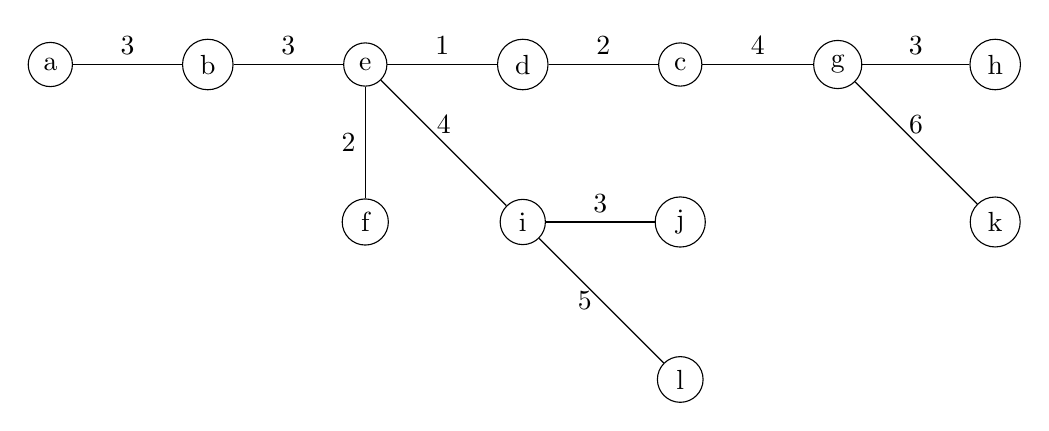
\begin{tikzpicture}
        \node[draw,circle] (a) at (0,0) {a};
        \node[draw,circle] (b) at (2,0) {b};
        \node[draw,circle] (e) at (4,0) {e};
        \node[draw,circle] (d) at (6,0) {d};
        \node[draw,circle] (c) at (8,0) {c};
        \node[draw,circle] (f) at (4,-2) {f};
        \node[draw,circle] (i) at (6,-2) {i};
        \node[draw,circle] (j) at (8,-2) {j};
        \node[draw,circle] (g) at (10,0) {g};
        \node[draw,circle] (h) at (12,0) {h};
        \node[draw,circle] (l) at (8,-4) {l};
        \node[draw,circle] (k) at (12,-2) {k};

        \draw (a) -- node[above] {3} (b);
        \draw (b) -- node[above] {3} (e);
        \draw (e) -- node[above] {1} (d);
        \draw (d) -- node[above] {2} (c);
        \draw (e) -- node[left] {2} (f);
        \draw (e) -- node[above] {4} (i);
        \draw (i) -- node[above] {3} (j);
        \draw (c) -- node[above] {4} (g);
        \draw (g) -- node[above] {3} (h);
        \draw (i) -- node[left] {5} (l);
        \draw (g) -- node[above] {6} (k);
    \end{tikzpicture}
    \caption{Minimum Spanning Tree generated using Prim's Algorithm}
\end{figure}

\newpage

\section*{Problem 2 (Kruskal's Algorithm)}
\begin{table}[ht]
    \centering
    \begin{tabular}{|c|c|}
        \hline
        \textbf{Tree Edges} & \textbf{Sorted List of Edges}                               \\
        \hline
                            & de(1) cd(2) ef(2) ab(3) be(3) gh(3) ij(3) ad(4) cg(4) ei(4) \\
                            & ac(5) dh(5) fj(5) il(5) bf(6) gk(6) hi(6) hk(7) kl(8) jl(9) \\
        \hline
        de(1)               & cd(2) ef(2) ab(3) be(3) gh(3) ij(3) ad(4) cg(4) ei(4)       \\
                            & ac(5) dh(5) fj(5) il(5) bf(6) gk(6) hi(6) hk(7) kl(8) jl(9) \\
        \hline
        cd(2)               & ef(2) ab(3) be(3) gh(3) ij(3) ad(4) cg(4) ei(4)             \\
                            & ac(5) dh(5) fj(5) il(5) bf(6) gk(6) hi(6) hk(7) kl(8) jl(9) \\
        \hline
        ef(2)               & ab(3) be(3) gh(3) ij(3) ad(4) cg(4) ei(4)                   \\
                            & ac(5) dh(5) fj(5) il(5) bf(6) gk(6) hi(6) hk(7) kl(8) jl(9) \\
        \hline
        ab(3)               & be(3) gh(3) ij(3) ad(4) cg(4) ei(4)                         \\
                            & ac(5) dh(5) fj(5) il(5) bf(6) gk(6) hi(6) hk(7) kl(8) jl(9) \\
        \hline
        be(3)               & gh(3) ij(3) ad(4) cg(4) ei(4)                               \\
                            & ac(5) dh(5) fj(5) il(5) bf(6) gk(6) hi(6) hk(7) kl(8) jl(9) \\
        \hline
        gh(3)               & ij(3) ad(4) cg(4) ei(4)                                     \\
                            & ac(5) dh(5) fj(5) il(5) bf(6) gk(6) hi(6) hk(7) kl(8) jl(9) \\
        \hline
        ij(3)               & ad(4) cg(4) ei(4)                                           \\
                            & ac(5) dh(5) fj(5) il(5) bf(6) gk(6) hi(6) hk(7) kl(8) jl(9) \\
        \hline
        cg(4)               & ad(4) ei(4)                                                 \\
                            & ac(5) dh(5) fj(5) il(5) bf(6) gk(6) hi(6) hk(7) kl(8) jl(9) \\
        \hline
        ei(4)               & ad(4)                                                       \\
                            & ac(5) dh(5) fj(5) il(5) bf(6) gk(6) hi(6) hk(7) kl(8) jl(9) \\
        \hline
        il(5)               & dh(5) fj(5)                                                 \\
                            & ac(5) bf(6) gk(6) hi(6) hk(7) kl(8) jl(9)                   \\
        \hline
        gk(6)               & hi(6) hk(7)                                                 \\
                            & ac(5) bf(6) kl(8) jl(9)                                     \\
        \hline

    \end{tabular}
    \caption{Kruskal's Algorithm to produce minimum spanning tree}
    \label{tab:table2}
\end{table}

\begin{figure}[h]
    \centering
    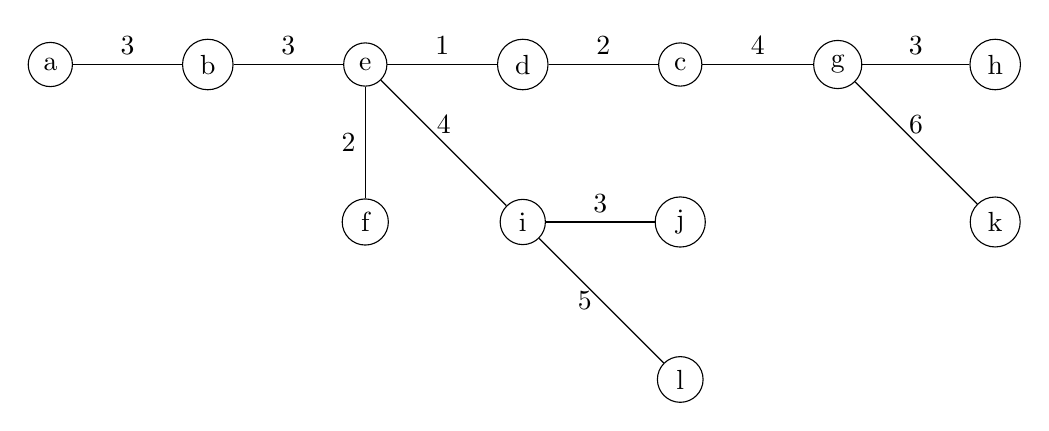
\begin{tikzpicture}
        \node[draw,circle] (a) at (0,0) {a};
        \node[draw,circle] (b) at (2,0) {b};
        \node[draw,circle] (e) at (4,0) {e};
        \node[draw,circle] (d) at (6,0) {d};
        \node[draw,circle] (c) at (8,0) {c};
        \node[draw,circle] (f) at (4,-2) {f};
        \node[draw,circle] (i) at (6,-2) {i};
        \node[draw,circle] (j) at (8,-2) {j};
        \node[draw,circle] (g) at (10,0) {g};
        \node[draw,circle] (h) at (12,0) {h};
        \node[draw,circle] (l) at (8,-4) {l};
        \node[draw,circle] (k) at (12,-2) {k};

        \draw (a) -- node[above] {3} (b);
        \draw (b) -- node[above] {3} (e);
        \draw (e) -- node[above] {1} (d);
        \draw (d) -- node[above] {2} (c);
        \draw (e) -- node[left] {2} (f);
        \draw (e) -- node[above] {4} (i);
        \draw (i) -- node[above] {3} (j);
        \draw (c) -- node[above] {4} (g);
        \draw (g) -- node[above] {3} (h);
        \draw (i) -- node[left] {5} (l);
        \draw (g) -- node[above] {6} (k);
    \end{tikzpicture}
    \caption{Minimum Spanning Tree generated using Kruskal's Algorithm}
\end{figure}




\end{document}